\documentclass{article}
\usepackage{enumitem}
\usepackage{pgf}
\usepackage{tikz}
\usepackage{tikz-cd}
\usepackage{listings}
\usepackage[utf8]{inputenc}
\usetikzlibrary{arrows, matrix}
\newcommand{\bold}{\textbf}
\newcommand{\itt}{\textit}
\newcommand{\tsc}{\textsc}
\newcommand{\vars}{\textit}
\newcommand{\cons}{\textrm}
\usepackage{textcomp}
\newcommand{\nothing}{{``nothing''}}
\long\def\RW#1{{\bf[RW: #1]}}
\long\def\NZ#1{{\sc[NZ: #1]}}
\lstdefinestyle{mystyle}{
    basicstyle=\footnotesize,
    breakatwhitespace=false,         
    breaklines=true,                 
    captionpos=b,                    
    keepspaces=true,                 
    numbers=left,                    
    numbersep=5pt,                  
    showspaces=false,                
    showstringspaces=false,
    showtabs=false,                  
    tabsize=2
}
\lstset{style=mystyle}

\begin{document}

\begin{titlepage}
   \vspace*{\stretch{1.0}}
   \begin{center}
      \Large\textbf{Characterization of Logging Usage:\\An Application of Discovering Infrequent Patterns via Anti-unification}
   \end{center}
   \vspace*{\stretch{2.0}}
\end{titlepage}

\begin{itemize} [leftmargin=.1in]
\item Determining the detailed structural similarities and differences between entities of the source code of a software system, or between the source code of different software systems, is a potentially complex problem
\item Being able to do so has various actual or potential applications%, such as code clone detection, automating source code reuse, recommending the replacements for an API migration, collating API usage patterns, and automating the merge operation in a version control system
\item As a specific application, our focus is on the study of where logging is used in the source code
\item logging is a pervasive practice and has various applications in software development and maintenance 
\item Developers have to make decisions about where and what to log
\item Logging should be done in an appropriate manner to be effective
\item Researches have often considered logging as a trivial task 
\item However, some evidence suggest that it is not a straightforward task to perform high quality logging in practice, such as:
\begin{itemize} 
\item availability of several complex frameworks to help developers to log  
\item the significant amount of effort developers spend to modify logging calls as after-thoughts [Yuan et al., 2012]
\end{itemize}
\item So far, little study has been conducted on understanding the usage of logging in real-world systems
\item \tsc{PROBLEM: }In this research, we would like to understand
where developers log in practice, in a detailed way
\item \tsc{SOLUTION: }Develop an automated approach to detect the detailed structural similarities and differences in the usage of logging within a system and between systems
\item \NZ{I am a little confused about how to find commonalities and differences of logging usage between systems? do you mean that I should compare the results taken from clustering of all Java classes in one system to another one?} \RW{The process of locating commonalities and differences can be applied within a single version of one system, across multiple versions of one system, across single versions of multiple systems, or across multiple versions of multiple systems.  It would be useful to understand the differences and similarities between different systems.  Is there some reason that this would be harder to achieve?} \NZ{I should think about it more. I can answer to this question after per-system analysis with more confidence}

\item \bold{Section 1.1 Broad thesis overview}
\item We aim to provide a concise description of where logging calls are used in the source code through creating generalizations that represent the detailed structural similarities and differences between Logged Java Classes (LJCs)

\item{Our approach:}
\begin{itemize}
\item applies a hierarchical clustering algorithm to classify LJCs into groups using a measure of similarity
\item uses an anti-unification algorithm to construct a structural generalization representing the similarities and differences of all LJCs in each group
\end{itemize}

\item{Our anti-unification approach:}
\begin{itemize}
\item uses the Jigsaw framework to determine all potential correspondences between a pair of LJCs
\item applies some constraints to avoid anti-unifying logged Java classes with non-logged Java classes
\item determines correspondences between structures containing logging calls by greedily applying a similarity measure to find the most similar substructures
\item develops a measure of structural similarity between LJCs
\end{itemize}
\item Our approach has been implemented as an Eclipse plug-in
\item An experiment is conducted on 10 sample LJCs to evaluate our approach and tool
\item To characterize logging usage, we applied our tool on the source code of three open-source software systems that make use of logging
\item Our experiment shows ...

\item \bold{Section 1.2 Overview of related work}
\item Yuan et al. [2012]  provides a quantitative characteristic study of log messages 
\item So far, anti-unification has been used for various applications:
\begin{itemize}
\item generalization task [Cottrell et al., 2007]
\item semi-automating small-scale reuse task[Cottrell et al., 2008]
\item Software clone detection [Bulychev and Minea, 2008]
\end{itemize}
\item This study makes the first attempt to characterize where logging calls occur through finding the detailed structural similarities and differences using anti-unification

\item \bold{Section 1.3 Thesis statement}
\item The thesis of this work is to determine the detailed structural similarities and differences between entities of the source code that make use of logging to provide a concise description of where logging do occur in real systems

\item \bold{Section 1.4 Thesis Organization}
\item Chapter 2: motivates the problem of understanding where to use logging calls in the source code through an example
\item Chapter 3: provides background information on ASTs, anti-unification and its extensions (HOAUMT), and the Jigsaw framework and why they matter in our study  
%\begin{itemize}
%\item abstract syntax trees (ASTs), which are the basic structure we will use for describing software source code
%\item how ASTs are realized in the Eclipse integrated development environment, the industrial tool we will build atop
%\item anti-unification and its limitations to solve our problem context
%\item higher-order anti-unification modulo theories (HOAUMT) that can be applied on an extended form of the AST structure to address our problem
%\item the Jigsaw framework, an existing tool for a subset of HOAUMT, which we extend to address our problem
%\end{itemize}
\item Chapter 4: describes our proposed approach and its implementation as an Eclipse plug-in
\item Chapter 5: presents an empirical study conducted to evaluate our approach and its application to characterize logging usage
\item Chapter 6: describes related work to our research problem and how it
does not adequately address the problem
\item Chapter 7: discusses the results and findings of my work, threats to its validity, and remaining issues
\item Chapter 8: concludes the dissertation, presents the contributions of this study, and future work

\item \bold{Chapter 2. Motivational Scenario}
\item Logging is a systematic way of recording the software runtime information
\item A typical logging call is composed of a log function and its parameters including a log message and verbosity level
\item Consider a developer is given the task of logging the Java class in Figure~\ref{ex1}
%\item She decides to use log4j framework for logging
\begin{figure}[H]
\def\baselinestretch{1}
\begin{lstlisting}
public class EditBus {
  private static ArrayList components=new ArrayList();
  private static EBComponent[] copyComponents;
  private EditBus(){
  
  public static void addToBus(  EBComponent comp){
    synchronized (components) {
      components.add(comp);
      copyComponents=null;
    }
  }
  public static void removeFromBus(  EBComponent comp){
    synchronized (components) {
      components.remove(comp);
      copyComponents=null;
    }
  }
  public static EBComponent[] getComponents(){
    synchronized (components) {
      if (copyComponents == null) {
        copyComponents=(EBComponent[])components.toArray(new EBComponent[components.size()]);
      }
      return copyComponents;
    }
  }
  public static void send(  EBMessage message){
    EBComponent[] comps=getComponents();
    for (int i=0; i < comps.length; i++) {
        EBComponent comp=comps[i];
        if (Debug.EB_TIMER) {
          long start=System.currentTimeMillis();
          comp.handleMessage(message);
          long time=(System.currentTimeMillis() - start);
        }
        else  comps[i].handleMessage(message);
    }
  }
}
\end{lstlisting}
\caption{A Java class without the usage of logging\label{ex1}}
\end{figure}

\item She has to make several decisions about
\begin{itemize}
\item what events need to be logged?
\item where to use logging calls?
\item how to decide on the log message and verbosity level of each logging call?
\end{itemize}
\item It is recommended to simply log at the start and end of every method
\item However, for example, logging at the start and end of the method \vars{addToBus} is useless, producing redundant information
\item She needs more information to perform logging appropriately
\item Having a characterization  of how usually developers use logging calls in similar situations would assist her in making decisions
\item For example, knowing that developers use logging calls inside of if statements to log a potential error when a variable contains an incorrect value, she adds an if statement to log an error when the value of the variable \vars{time} is \vars{null} (shown in Lines~36-38 of Figure~\ref{ex2})
\item For example, knowing that developers use logging calls inside catch blocks to record an exception, she creates a try/catch block to capture the potential failure in sending messages and uses a logging call in the catch block (Lines~41-43 of Figure~\ref{ex2})

\begin{figure}[H]
\def\baselinestretch{1}
\begin{lstlisting}
public class EditBus {
 private static ArrayList components=new ArrayList();
  private static EBComponent[] copyComponents;
  private EditBus(){
  }
  public static void addToBus(  EBComponent comp){
    synchronized (components) {
      components.add(comp);
      copyComponents=null;
    }
  }
  public static void removeFromBus(  EBComponent comp){
    synchronized (components) {
      components.remove(comp);
      copyComponents=null;
    }
  }
  public static EBComponent[] getComponents(){
    synchronized (components) {
      if (copyComponents == null) {
        copyComponents=(EBComponent[])components.toArray(new EBComponent[components.size()]);
      }
      return copyComponents;
    }
  }
  public static void send(  EBMessage message){
    Log.log(Log.DEBUG,EditBus.class,message.toString());
    EBComponent[] comps=getComponents();
    for (int i=0; i < comps.length; i++) {
      try {
        EBComponent comp=comps[i];
        if (Debug.EB_TIMER) {
          long start=System.currentTimeMillis();
          comp.handleMessage(message);
          long time=(System.currentTimeMillis() - start);
          if (time != 0) {
             Log.log(Log.DEBUG,EditBus.class,comp + ": " + time+ " ms");
          }
        }
        else  comps[i].handleMessage(message);
      }catch (Throwable t) {
         Log.log(Log.ERROR,EditBus.class,"Exception" + " while sending message on EditBus:");
      }
    }
  }
}
\end{lstlisting}
\caption{A Java class after the usage of logging calls\label{ex2}}
\end{figure}

\item Using a concise characterization she would be able to make informed decisions about where to use logging calls more easily and quickly
\item With taking appropriate decisions about where to use logging calls, she can spend more time and energy to write the context of log functions% and even other development and maintenance tasks

\item \bold{Chapter 3. Background}
\item \bold{Section 3.1. Abstract Syntax Tree}
\item The Eclipse Java Development Tools (JDT) framework provides APIs to access and manipulate Java source code via Abstract Syntax Tree (AST)
\item AST maps Java source code in a tree structure form
%\item Every Java source code can be represented as tree of AST nodes
%\item Every AST node represents an element of the Java Programming Language
\item Structural properties of an AST node hold specific information for the Java element it represents
\item Structural properties are stored in a map data structure that associates each property to its value
\item The structural properties have three different types:
\begin{itemize} [leftmargin=.1in]
\item \itt{Simple Property:} where the value is an AST constant (simple value)
\item \itt{Child Property:} where the value is a single AST node
\item \itt{Child list property:} where the value is a list of AST nodes
\end{itemize}
%\item AST nodes are subtrees of the tree structure and simple values are the leaves

\item \bold{Section 3.2. Anti-unification}
\item  A \itt{term} is a set of
\begin{itemize} [leftmargin=.1in]
\item \itt{Function symbols} (e.g., \vars{f(a,b)})
\item \itt{Constants} (e.g. \vars{a})
\item \itt{Variables} (e.g., \vars{X})
\end{itemize}
\item \itt{Ground term}: a term that does not contain any variables 
\item A \itt{Substitution} is defined on a term to map its variables to ground terms
\item \itt{Applying Substitutions}: replacing all occurrences of a variable with a proper term
\item \itt{Instance \& Anti-Instance }:  \vars{a} is an instance of \vars{X} and \vars{X} is an anti-instance of \vars{a}, if there is a substitution $\ominus$ such that the application of $\ominus$ on \vars{X} results in \vars{a} (\begin{tikzcd}[column sep=small] \vars{X} \arrow[r,->,shift right,"\ominus"] & \vars{a} \end{tikzcd})
\item \itt{Unifier}: A common instance of two given terms
\item \itt{Most General Unifier (MGU)}: \vars{U} is MGU of two structures such that for all unifiers \vars{U}${\prime}$ there exist a substitution $\ominus$ such that \begin{tikzcd}[column sep=small] \vars{U} \arrow[r,->,shift right,"\ominus"] & \vars{U$\prime$} \end{tikzcd}

\item \itt{Generalization}: \vars{X} is a generalization for \vars{a} and \vars{b}, where \vars{X} is an anti-instance for  \vars{a} and \vars{b} under substitutions $\ominus_1$ and $\ominus_2$, respectively. (\begin{tikzcd}[column sep=small] \vars{X} \arrow[r,->,shift right,"\ominus_1"] & \vars{a} \end{tikzcd} and\begin{tikzcd}[column sep=small] \vars{Y} \arrow[r,->,shift right,"\ominus_2"] & \vars{b} \end{tikzcd})

\item \itt{Anti-unifier}: A common generalization of two given terms
\item \itt{Most Specific Anti-unifier (MSA):} \vars{A} is MSA of two structures where there exist no anti-unifier \vars{A}${\prime}$ such that\begin{tikzcd}[column sep=small] \vars{A} \arrow[r,->,shift right,"\ominus"] & \vars{A$\prime$} \end{tikzcd}
\item MSA should preserve as much of structure of both original structures as possible
\item \itt{Anti-unification}: The process of finding the MSA of two given terms
\item \itt{First-order anti-unification}: restricts substitutions to replace only first-order variables by terms

\item \tsc{PROBLEM:} First-order anti-unification fails to capture complex structural commonalities
% anti-unifier always exist
\item \tsc{SOLUTION:} Higher-order anti-unification allow the creation of MSA by extending the set of possible substitutions such that variables can be replaced by not only constants but also functional symbols

\item An instance of an AST structure can be mapped  to our recursive definition of a term, where AST nodes and simple values may be viewed as function-symbols and constants, respectively

\item A set of equivalence equations is defined to incorporate semantic knowledge of structural equivalences supported by the Java language specification
\item These equational theories are applied on higher-order extended structures to allow the anti-unification of AST structures that are not identical but are semantically equivalent

\item The NIL structure is defined to create a structure out of nothing that would allow the anti-unification of two structures when a substructure exist in one but not in the other one

\item Defining complex substitutions results in losing the uniqueness of MSA
\item The complexity of finding an MSA is undecidable in general since an infinite number of substitutions can be applied on every variable in a structure
\item Our goal is to find an MSA that is an approximation of the best fit to our application

\item \bold{Section 3.3. Jigsaw}
\item The Jigsaw tool is developed by Cottrell et al. [2008] to determine the structural correspondences between two Java source code fragments through anti-unification such that one fragment can be integrated to the other one for small scale code reuse
\item The Jigsaw framework could help us to construct an anti-unifier form logged Java classes as it:
\begin{itemize}
\item applies higher-order anti-unification modulo theories to address the limitations of first-order syntactical anti-unification
\item creates an augmented form of AST, called CAST (Correspondence AST), in which each node holds a list of candidate correspondence connections between the two structures, each representing an anti-unifier
\item develops a measure of similarity to indicate how similar the nodes involved in one correspondence connection are

\end{itemize}
\item The Jigsaw similarity function:
\begin{itemize}
\item returns a value between 0 and 1 where indicate zero and total matching, respectively
\item uses several semantical heuristics to improve the accuracy of similarity measurement
\end{itemize}
\item The Jigsaw tool does not sufficiently solve our problem since:
\begin{itemize}
\item it determines all potential correspondences between AST nodes, each representing an anti-unifier; however, we need to determine one single anti-unifier% that is approximately the best fit to our problem
\item it does not construct an anti-unifier of two given AST structures with a focus on logging calls%, which is required to our application
\end{itemize}

\item \bold{Chapter 4. Anti-unification of Logged Java Classes}
\item \bold{Section 4.1. Constructing an anti-unifier}
\item \tsc{Problem: }constructing an anti-unifier (structural generalization) from two given logged Java classes with a special  attention to logging calls

\begin{figure} [H]
  \centering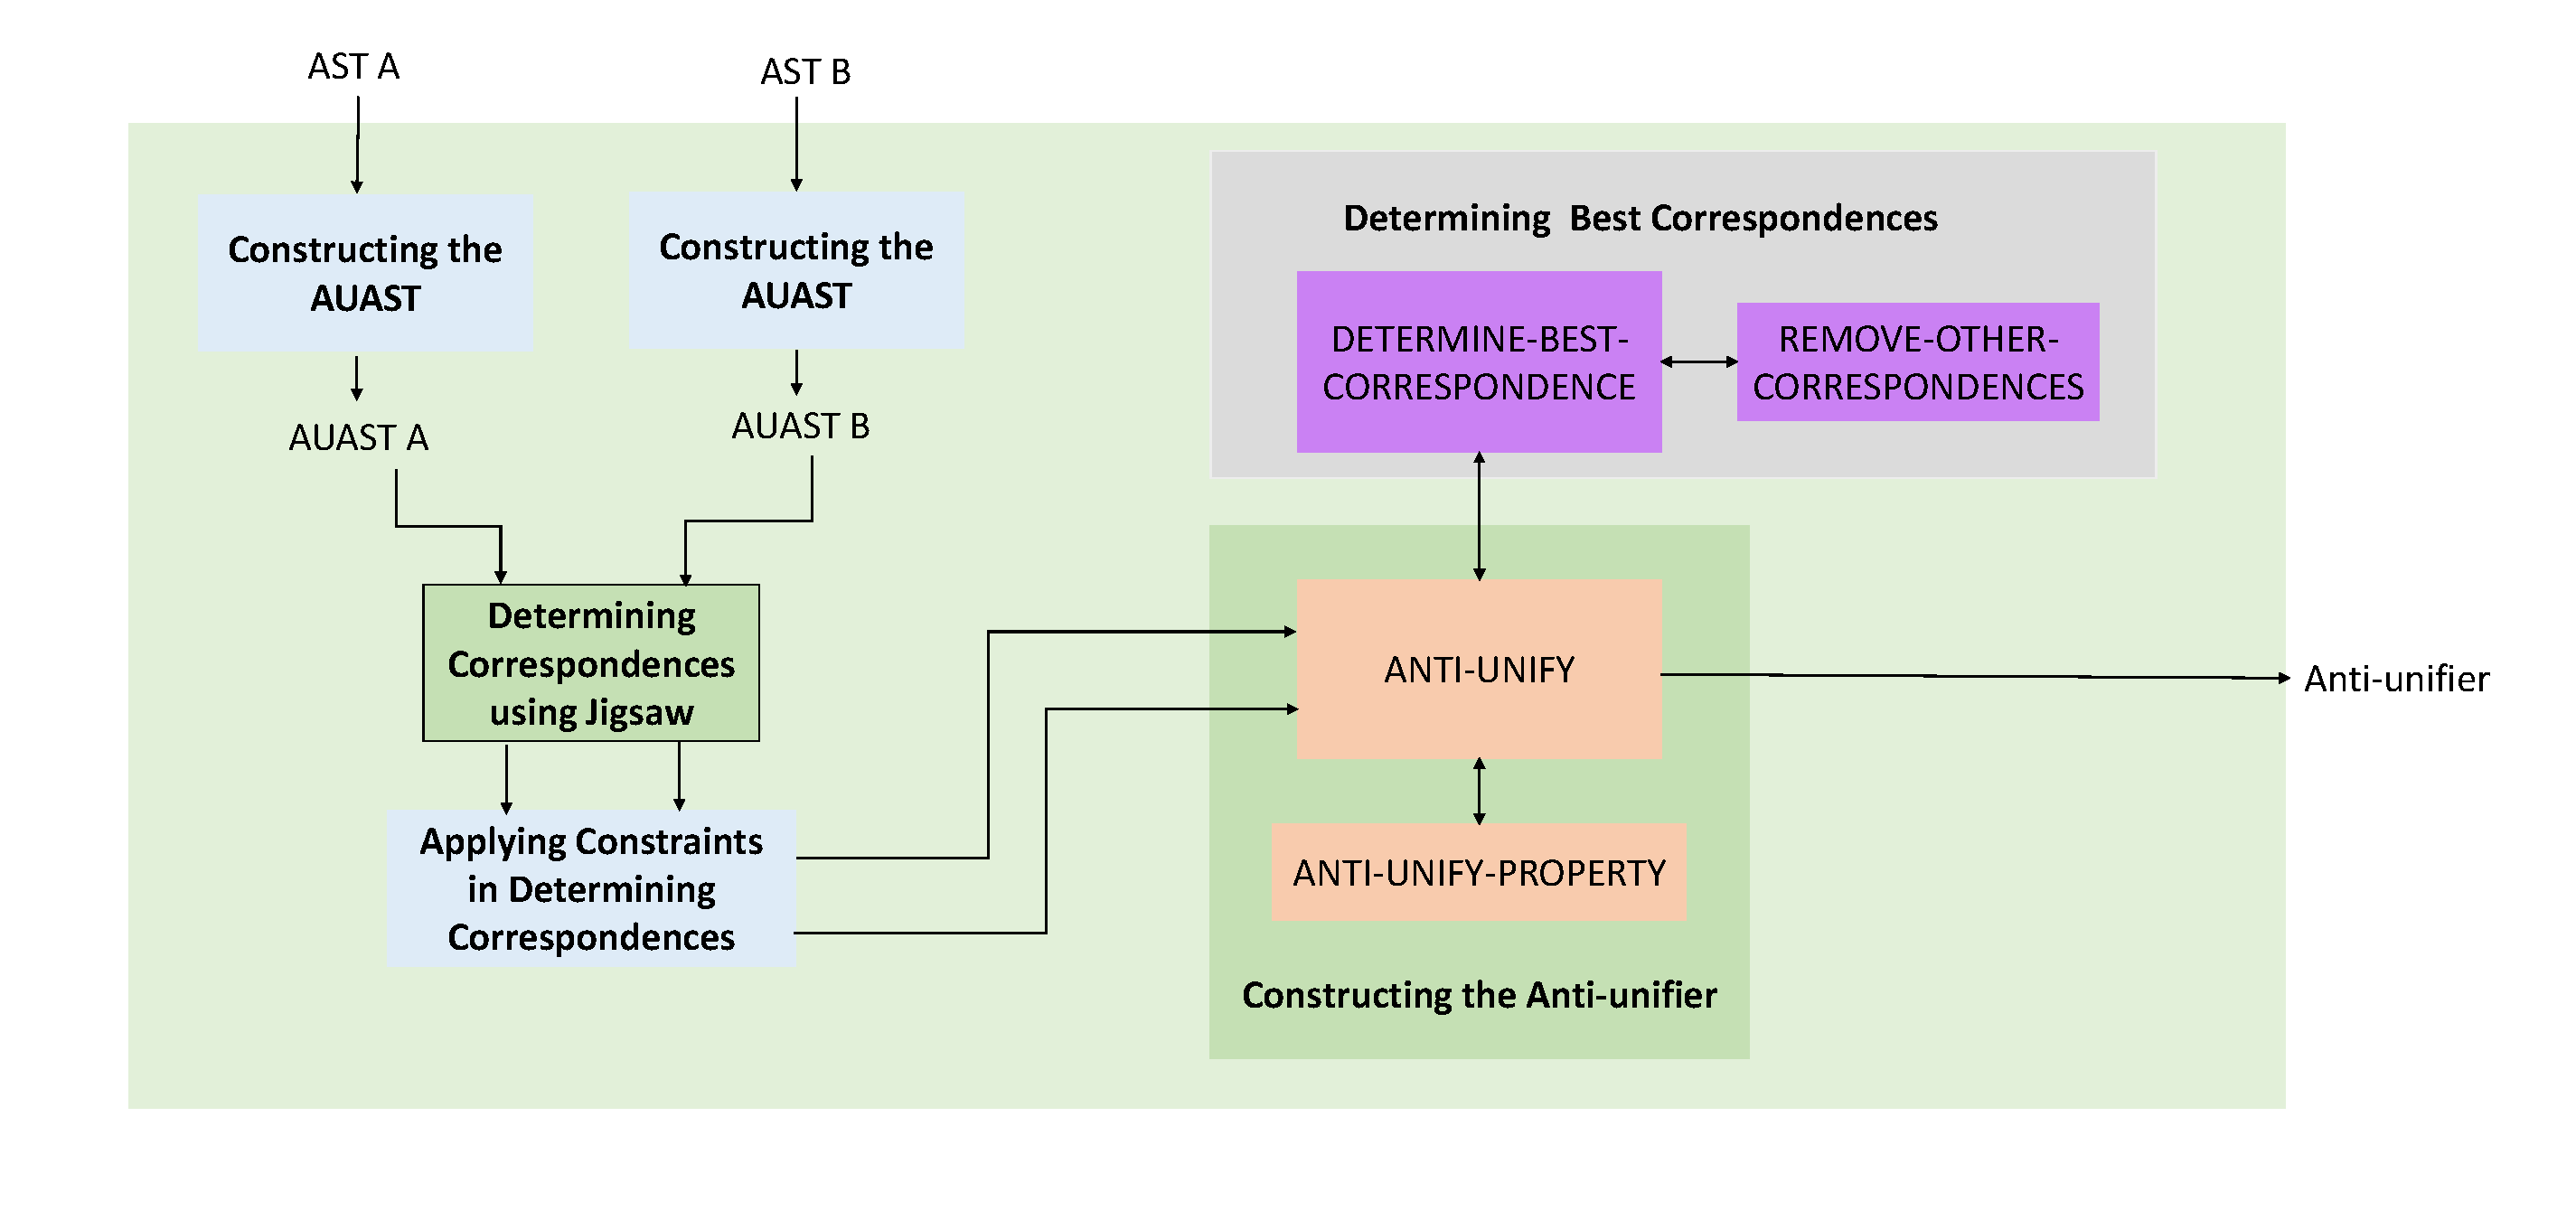
\includegraphics [width = \textwidth]{Drawing4/overview1.pdf}
  \caption{Overview of the approach for constructing an anti-unifier}
  \label{fig:overview1}
\end{figure}

\item \tsc{Solution: } Developing an Algorithm (depicted in Figure~\ref{fig:overview1}) that:
\begin{itemize} [leftmargin=.1in]
\item maps the source code of two LJCs to AST structures via the Eclipse JDT framework 
\item creates an extension of AST structures, called AUAST, to allow the insertion of variables in place of any nodes 
\item determines potential candidate structural correspondences between AUAST nodes using the Jigsaw framework 
\item applies some constraints to prevent the anti-unification of logging calls with anything else 
\item determines the best structural correspondences between AUAST nodes to handle the problem of having multiple anti-unfiers using a greedy selection algorithm
\item constructs an anti-unifier through anti-unification of structural properties
\item develops a measure of similarity between the two AUASTs 
\end{itemize}

\item \bold{Chapter 4.2 Anti-unifying a set of LJCs}
\item \tsc{Problem: } anti-unifying a set of AUASTs of LJCs
\item \tsc{Solution: }Developing a modified version of a hierarchical agglomerative clustering algorithm (illustrated in Figure~\ref{fig:overview2}) as described below: 
\begin{enumerate}
\item Start with singleton clusters, where each cluster contains one AUAST 
\item Compute the similarity between clusters in a pairwise manner 
\item Find the closest clusters (a pair of clusters with maximum  similarity)
\item Merge the closest cluster pair and replace them with a new cluster containing anti-unifier of AUASTs of the two clusters 
\item Compute the similarity between the new cluster and all remaining clusters 
\end{enumerate}
\begin{itemize}
\item Repeat Steps 3,4, and 5 until the similarity between closest clusters becomes below a predetermined threshold value
\item The similarity between a pair of clusters is defined as the similarity between their AUASTs 
\item Determine the similarity threshold value through informal experimentation 
\end{itemize}
\begin{figure} [H]
  \centering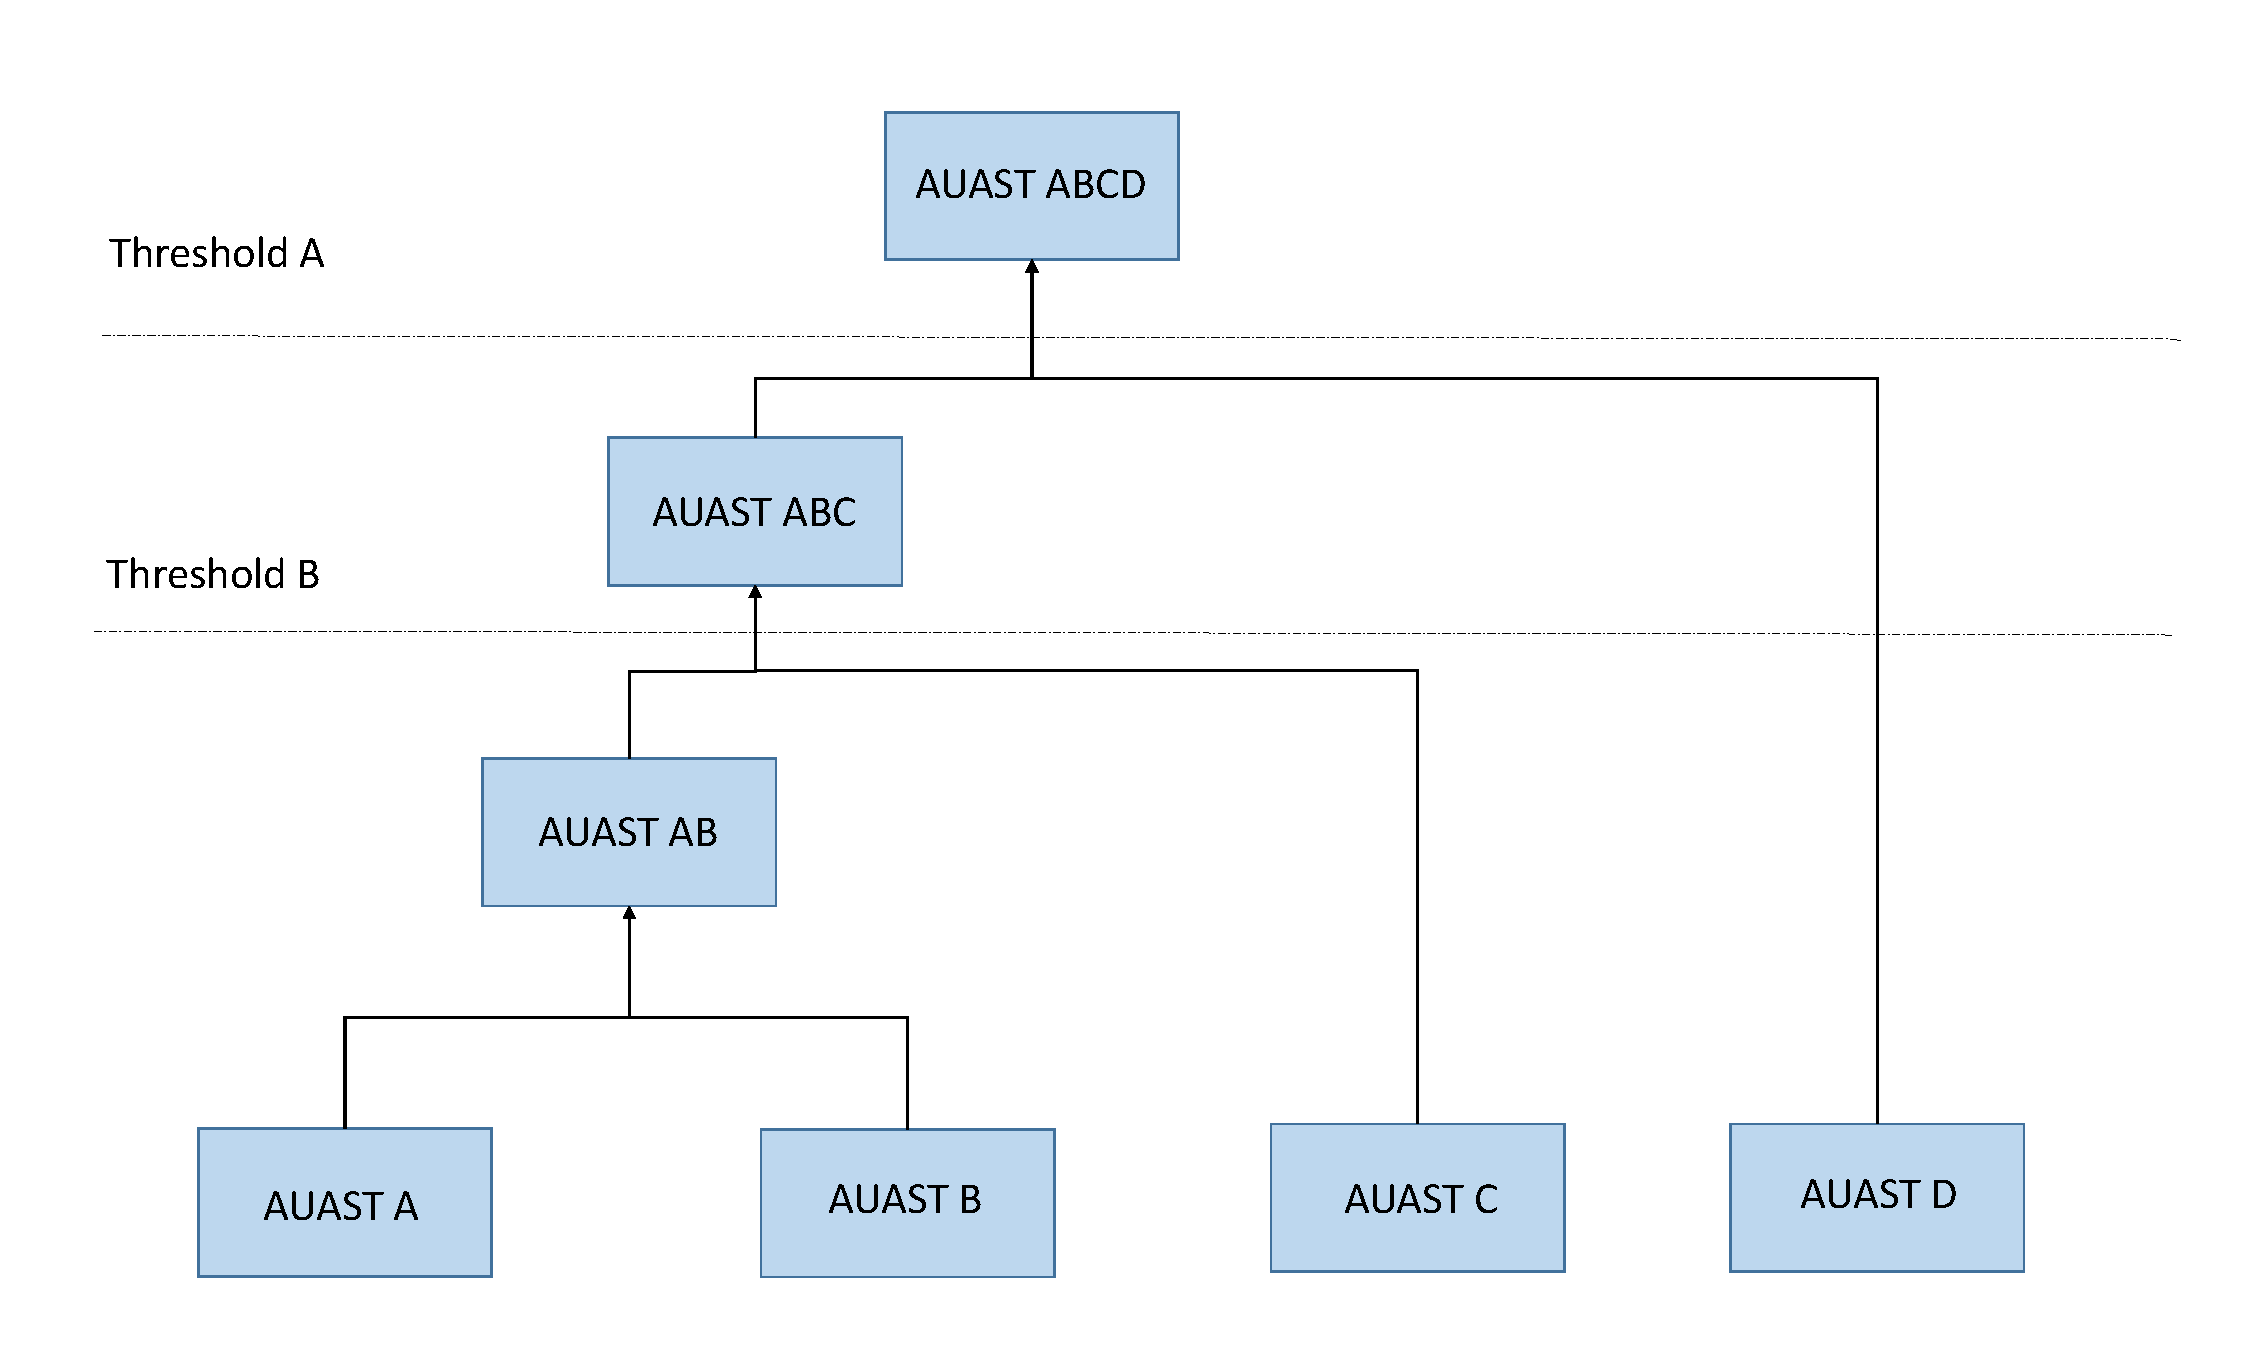
\includegraphics [width = \textwidth]{Drawing4/overview2.pdf}
  \caption{Anti-unification of 4 AUAST nodes using an agglomerative hierarchical clustering algorithm. Each rectangle is an indicator of a cluster. The threshold value indicates the number of clusters we will come up with.}
  \label{fig:overview2}
\end{figure}

\item \bold{Chapter 5. Evaluation}
\item Two empirical studies were conducted
\item \bold{Section 5.1 Experiment 1}
\item First experiment is conducted to evaluate the accuracy of our approach and tool
\item It addresses the following research questions:
\begin{itemize}
\item \tsc{RQ1: }can our tool determine the structural similarities and differences between LJCs correctly?
\item \tsc{RQ2: }can our tool compute the similarity between LJCs correctly?
\end{itemize}
\item 10 logged Java classes were selected randomly from jEdit v4.2 pre 15 (2004), as our test set
\item We apply our tool on the test set to create generalizations  and to compute the similarity between LJCs in a pairwise manner
\item To address the first research question we compute the following measurements for each test case:
\begin{itemize}
\item the number of correspondences that our tool detects correctly
\item the total number of correspondences
\end{itemize}
\item To determine the correct correspondences we performed a manual investigation
\item To address the second research question we compute:
\begin{itemize}
\item the number of similarity values between logged Java classes that are computed correctly by our tool
\item the total number of comparisons
\end{itemize}
%\item The correct similarity value for each comparison is calculated manually by
%\begin{itemize}
%\item counting common simple values based on the selection of corresponding AUAST nodes
%\item counting total number of simple values of AUAST nodes
%\end{itemize}
\item The results taken form our tool are compared with the results taken by manual investigation using the JUnit testing framework

\item \bold{Section 5.2 Experiment 2}
\item Second experiment is conducted to address the following research questions:
\begin{itemize}
\item \tsc{RQ3: }What structural similarities and differences do logged Java classes have?
\item \tsc{RQ4: }Is it possible to find common patterns in where logging calls do occur?
\end{itemize}
\item We applied our tool on the source code of three open-source full systems that make use of logging to determine the patterns on a per-system class-granularity basis analysis
%\item These systems are different from the system that the test set is selected from
\item \bold{Section 5.2.1 Results}
\item ...
\item \bold{Section 5.2.2 Lessons learned}
\item ...

\item \bold{Chapter 6. Discussion}
\item \bold{Chapter 6.1 Threats to validity}
%\item Our goal is to recognize the limitations and pitfalls of our approach and its developed tool support 
\item Some potential threads to validity of our characterization study are:
\begin{itemize}
\item the degree to which our sample set of software systems is a good representation of all real-world logging practices
\item the potential bias in our manual investigation to find the correct correspondences due to human errors
\end{itemize}
\item \bold{Chapter 6.2 Our tool output}
\item We found that the failures of our tool happen due to:
\begin{itemize}
\item the assumptions taken in developing the algorithms
\item the fundamental limitations and complexities in determining the detailed structural similarities and differences 
\end{itemize}

\item The are some issues that our tool is not able to handle perfectly during generalization:
\begin{itemize} 
\item maintaining the correct ordering of statements inside the method bodies
\item resolving all the conflicts that happen in determining the best correspondences
\item producing executable generalizations
\end{itemize}
\item However, these results are still promising

\item \bold{Chapter 6.3 Theoretical foundation}
\item Anti-unification and its extensions has several theoretical and practical applications: 
\begin{itemize}
\item analogy making [Schmidt, 2010]
\item determining lemma generation in equational inductive proofs [Burghardt, 2005]
\item detecting the construction laws for a sequence of structures [Burghardt, 2005]
\end{itemize}
%\item Using higher-order anti-unification modulo theories in our application, which is undecidable in general, leads us to take approximations suitable to our context
\item The set of equational theories in HOAUMT should be developed particularly for the structure used in each problem context 

\item \bold{Chapter 7. Related Work}
\item \bold{Section 7.1 Logging}
\item Logging is a systematic way of recording the software runtime information [Yuan et al., 2012]
\item It has various applications, such as:
\begin{itemize}
\item problem diagnosis[Jiang et al., 2009a and Jiang et al. 2009b]
\item system behavioural understanding [Fu et al., 2013 and Yaghmour et al., 2000]   
\item performance diagnosis [Nagaraj et al., 2012] 
\item system\textquotesingle s security monitoring [Bishop, 1989]
\item system\textquotesingle s recovery [Elnozahy et al. 2002] 
\end{itemize}
\item Yuan et al. [2012]  provides a quantitative characteristic study of log messages
\item Their study shows: 
\begin{itemize}
\item logging is a pervasive practice during software development
\item developers are not mostly satisfied with the log quality in their first attempt
\item where developers spend most of their time in modifying the log messages
\end{itemize}
\item However, the focus of our study is on characterizing where developers log (not the log messages)

\item \bold{Section 7.2 Correspondence}
\item Anti-unification, which is first introduced by Plotkin [1970] and Reynolds [1970], has various applications in program analysis, such as: 
\begin{itemize}
\item software clone detection[Bulychev and Minea, 2008]
\item generalization tasks [Cottrell et al., 2007]
\item semi-automating small scale reuse tasks [Cottrell et al., 2007]
\item recommending replacements for API migration [Bradley et al., 2014]
\end{itemize}
\item These studies utilize anti-unification to detect structural correspondences between the source code fragments, however, none of them suffice to our problem context since they:
\begin{itemize}
\item do not require to take constraints needed to our problem
\item do not determine the best correspondences required to our application
\item do not create the structural generalizations needed to our context
\end{itemize}
\item Several other approaches have been used to find correspondences between code fragments [Baxter et al. 1998, Apiwattanapong et al., 2004, Holmes et al., 2006, Sager et al., 2006] 
\item However, these approaches do not determine the detailed structural similarities and differences needed in our context 


\item \bold{Section 7.4 API usages patterns}
\item Various data mining approaches has been used to extract API usages patterns, such as 
\begin{itemize}
\item association rule mining [Michail , 2000]
\item itemset mining [Li and Zhou, 2005]
\item sequential pattern mining[Xie and Pei, 2006]
\end{itemize}
\item However, none of these approaches suffice to our context since they do not determine the detailed structural similarities and differences needed in our context

\item \bold{Section 7.5 Clustering}
\item Clustering is an unsupervised machine mining technique that aims to organize a collection of data into clusters, such that intra-cluster similarity is maximized and the inter-cluster similarity is minimized [Karypis, 1999] [Grira et al., 2004]
\item Clustering methods:
\begin{itemize}
\item K-means [Hartigan et al., 1979]
\begin{itemize}
\item Not a good fit to our problem since it requires to define a fixed number of clusters
\end{itemize}
\item Hierarchical clustering [Rasmussen, 1992]
\begin{itemize}
\item The cut-off threshold value indicates the number of clusters we will come up with
\end{itemize}
\end{itemize}
\item Agglomerative hierarchical clustering is one of the main stream clustering methods [Day, 1984] and has applications in:
\begin{itemize}
\item document retrieval [Voorhees, 1986]
\item information retrieval from a search engine query log [Beeferman et al., 2000]
\end{itemize}
%\item There are various techniques to measure the distance between clusters [Rasmussen, 1992]:
%\begin{itemize}
%\item Single linkage
%\item Complete linkage
%\item Average linkage
%\item Centroids
%\item Ward's method
%\end{itemize}
%\item However, in our application, the distance between clusters is defined as the distance between their AUAST nodes

\item \bold{Chapter 8. Conclusion}
\item Determining the detailed structural similarities and differences between source code fragments is a complex task
\item It can be applied to solve several source code analysis problems, for example, characterizing logging practices
\item logging is a pervasive practice and has various applications in software development and maintenance
\item However, it is a challenging task for developers to understand how to use logging calls in the source code 
\item We have presented an approach to characterize where logging calls happen in the source code by means of structural generalizations
\item We have developed a prototype tool that: 
\begin{itemize}
\item detects potential structural correspondences using anti-unification
\item uses several constraint to remove the correspondences that are not suited to our application 
\item determines the best correspondences with the highest similarity
\item constructs structural generalizations using anti-unification
\item classifies the entities using a measure of similarity 
\end{itemize}
\item An experiment is conducted to evaluate our approach and tool
\item Our experiment found that ... 
\item An experiment is conducted to characterize logging usage in three software systems
\item In summary, our study makes the following contributions:
\begin{itemize}
\item …
\item …
\end{itemize}

\item \bold{Section 8.1 Future Work} 
\item Future extensions could be applied to resolve the pitfalls of this study:
\begin{itemize}
\item Data flow analysis techniques: to resolve the problem of inaccurate statement ordering
\item Further analysis: to detect and resolve all the conflicts happen in deciding the best correspondences
\end{itemize}
\item However, the complexity of further analysis should be limited to keep the solution practical 
\item A survey can be conducted to further validate our findings
\item Characterizing logging usage could be a huge step towards:
\begin{itemize}
\item improving the quality of logging practices %by providing some guidelines that might help developers in making decisions about where to log.
\item developing recommendation support tools to save developers\textquotesingle time and effort 
\end{itemize}

\end{itemize} %chapters
\end{document} 